\section{\texorpdfstring{CO$_2$}{CO2} Meter}

If we assume that the data follows an exponential plateau, approaching some steady state value C, then that means for any $t$ our expected $y$ (concentration in ppm) is
\begin{align*}
    y(t) = C - B e^{-At}
\end{align*}

To include the error as a fit parameter, let's say (since we have no other reason to pick a different distribution) that for every $t$ we have a Gaussian distribution with mean $\mu = C - B e^{-At}$ and standard deviation $\sigma_y$.

With that, we can do a maximum likelihood fit.

\begin{align*}
    L &= \prod_i P(y(t_i)=y_i) \\
    -\ln(L) &= -\ln(\prod_i P(y(t_i)=y_i)) \\
    -\ln(L) &= \sum_i -\ln(P(y(t_i)=y_i)) \\
\end{align*}

I fit this numerically, and got the results here:

\begin{align*}
    C &= 923 \\
    B &= 440 \\
    A &= 0.008875\\
    \sigma_y &= 2.77 \\
\end{align*}

A plot just to make sure the fit is reasonable:
\begin{figure}[H]
    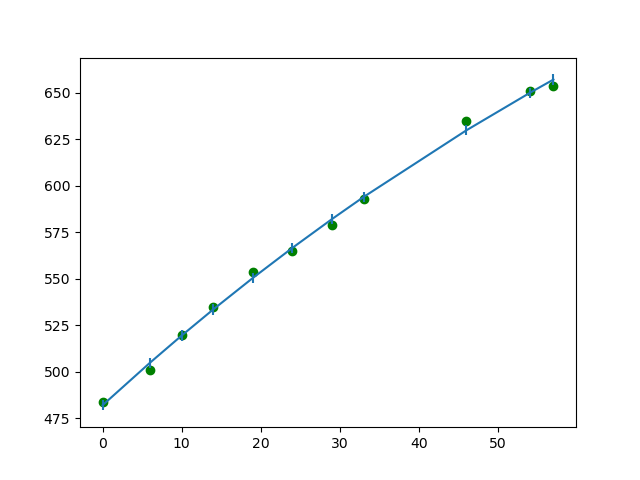
\includegraphics[width=\textwidth]{q3.png}
\end{figure}

Then how much of that is due to error in $t$?

Well if the error in $t$ is 1 minute, then the error in the exponential is given as follows (using error propagation equations):

\begin{align*}
    E &= e^{-At} \\
    \sigma_E &= Ae^{-At}\sigma_t \\
\end{align*}

If we use $\sigma_t = 1$ (minute) and $A=0.008875$ from before, evaluated at the minimum measured $t$ to maximize uncertainty, i.e. $t=0$, we get the uncertainty from $t$ is $A=0.008875$.

